\documentclass[conference]{IEEEtran}
\IEEEoverridecommandlockouts
% The preceding line is only needed to identify funding in the first footnote. If that is unneeded, please comment it out.
%Template version as of 6/27/2024

\usepackage{cite}
\usepackage{amsmath,amssymb,amsfonts}
\usepackage{algorithmic}
\usepackage{graphicx}
\usepackage{textcomp}
\usepackage{xcolor}
\usepackage{booktabs}
\usepackage{framed}
\def\BibTeX{{\rm B\kern-.05em{\sc i\kern-.025em b}\kern-.08em
    T\kern-.1667em\lower.7ex\hbox{E}\kern-.125emX}}
% Highlighted notes on what each part should cover. Before submission, hide
% them all by changing the definition to: \newcommand{\guide}[1]{}
% The shaded box (framed package) breaks across columns and pages, so a long
% note never runs off the bottom of a page.
\colorlet{shadecolor}{yellow!35}
\setlength{\FrameSep}{3pt}
\newcommand{\guide}[1]{\par\vspace{2pt}\begin{shaded}\normalfont\footnotesize\noindent #1\end{shaded}\par}
\begin{document}

\title{SimGate: An AI Agent That Runs\\Stress Testing of a Driving Policy
\thanks{Identify applicable funding agency here. If none, delete this.}
}

\author{\IEEEauthorblockN{1\textsuperscript{st} Given Name Surname}
\IEEEauthorblockA{\textit{dept. name of organization (of Aff.)} \\
\textit{name of organization (of Aff.)}\\
City, Country \\
email address or ORCID}
\and
\IEEEauthorblockN{2\textsuperscript{nd} Given Name Surname}
\IEEEauthorblockA{\textit{dept. name of organization (of Aff.)} \\
\textit{name of organization (of Aff.)}\\
City, Country \\
email address or ORCID}
\and
\IEEEauthorblockN{3\textsuperscript{rd} Given Name Surname}
\IEEEauthorblockA{\textit{dept. name of organization (of Aff.)} \\
\textit{name of organization (of Aff.)}\\
City, Country \\
email address or ORCID}
\and
\IEEEauthorblockN{4\textsuperscript{th} Given Name Surname}
\IEEEauthorblockA{\textit{dept. name of organization (of Aff.)} \\
\textit{name of organization (of Aff.)}\\
City, Country \\
email address or ORCID}
\and
\IEEEauthorblockN{5\textsuperscript{th} Given Name Surname}
\IEEEauthorblockA{\textit{dept. name of organization (of Aff.)} \\
\textit{name of organization (of Aff.)}\\
City, Country \\
email address or ORCID}
\and
\IEEEauthorblockN{6\textsuperscript{th} Given Name Surname}
\IEEEauthorblockA{\textit{dept. name of organization (of Aff.)} \\
\textit{name of organization (of Aff.)}\\
City, Country \\
email address or ORCID}
}

\maketitle

\begin{abstract}
\guide{About 150 words, written last, with the final numbers. Four sentences: (1) the problem: stress testing an end-to-end driving policy in closed loop takes thousands of runs; by hand it is slow, and left unattended it fails silently; (2) what SimGate is: an AI agent that runs the whole campaign, choosing only from fixed menus that code checks and scripts carry out; (3) the evidence: the scale of the unattended campaign, the share of failed launches healed with no person, and that no planted invalid run was kept; (4) the main finding: where failures are rare, letting the agent choose the next tests confirms the hardest cases sooner than rules, random search or Optuna.}
\end{abstract}

\begin{IEEEkeywords}
\guide{Four to six index terms covering autonomous vehicle testing, stress testing, LLM agents and closed-loop simulation.}
\end{IEEEkeywords}

% ---------------------------------------------------------------------------
\section{Introduction}\label{sec:intro}
\guide{\textbf{Paragraph 1: background and gap.} Motivate accelerated stress testing of end-to-end driving policies~\cite{feng2021nade,feng2023d2rl}, now possible in closed loop on real recorded scenes with neural-reconstruction simulators~\cite{ljungbergh2024neuroncap,zhou2024hugsim,alpasim}. State the gap: a campaign is thousands of runs that someone must choose, relaunch when they crash, and verify; left unattended it fails silently (use concrete early examples: a misconfigured model, a delay that never applied, missing results), and simulation results can themselves be flaky or nondeterministic ~\cite{osikowicz2025flaky,amini2024flaky,chance2022determinism}. Then the second half of the gap: handing the campaign to an AI agent that acts in a fully closed loop does not fix this by itself. An evaluation of an AI-scientist system found many experiments failing and hallucinated numbers in its papers~\cite{beel2025sakana}; such systems hide pitfalls that only full trace logs reveal~\cite{luo2025pitfalls}; coding agents make checks pass by deleting failing tests~\cite{zhong2025impossiblebench}; data-analysis agents finish without error yet answer the wrong question~\cite{yan2026failloudly}. Checking has not kept pace with what agents produce~\cite{mo2026trustworthy}.}

\guide{\textbf{Paragraph 2: approach and core contributions.} Open with the approach: hand the whole campaign to an AI agent but never let it decide what counts: it only proposes from fixed menus, code checks every proposal and every run, and every failure is kept with its evidence. Then list the contributions, each naming where it is described and where it is validated. (1) An agent that runs stress testing of an end-to-end driving policy end to end and unattended, in a neural-reconstruction simulator (Sec.~\ref{sec:method}; Sec.~\ref{sec:healing}). (2) An action design that makes it trustworthy: every job is a contract with a fixed menu, checked by code and carried out by scripts; the recovery menu is checked exhaustively, and every kept run is verified against its request (Sec.~\ref{sec:overview}, \ref{sec:gate}, \ref{sec:diagnose}; Sec.~\ref{sec:validity}). (3) Evidence that letting the agent choose the next tests confirms the hardest cases sooner where failures are rare, at an equal budget against rules, random search and Optuna (Sec.~\ref{sec:outer}; Sec.~\ref{sec:discovery}). (4) Results a person can check: every failure the agent handled with its evidence, a case card for every confirmed hardest case, and the agent's failure explanations checked against rules and people (Sec.~\ref{sec:healing}, \ref{sec:triage}, \ref{sec:cases}). Do not claim to be the ``first''.}

\guide{\textbf{Paragraph 3: organization of the paper.} One sentence per section. Sec.~\ref{sec:related} reviews accelerated stress testing, LLMs in scenario generation and testing, and agents that act safely. Sec.~\ref{sec:method} presents the framework around Fig.~\ref{fig:system}: its overview, the outer loop that plans a study and chooses the next runs, the inner loop that checks each run and heals failed ones, and how a study closes with triage and a report. Sec.~\ref{sec:results} describes the simulation setup and validates the framework: the validity of kept runs, self-healing in unattended operation, corner-case discovery across search methods, the reliability of failure triage, and the failures found in the policy under test. Sec.~\ref{sec:conclusion} concludes with limitations and future work.}

% ---------------------------------------------------------------------------
\section{Related Work}\label{sec:related}
\guide{Three short paragraphs. (1) Accelerated and adaptive stress testing (NADE~\cite{feng2021nade}, D2RL~\cite{feng2023d2rl}, adaptive stress testing~\cite{lee2020ast,koren2018ast}, Bayesian optimization~\cite{abeysirigoonawardena2019adversarial,osikowicz2026mfbo}): they supply search algorithms; this paper studies who chooses the next test and how a campaign stays valid. (2) LLMs in scenario generation and testing (LLM-attacker~\cite{mei2025llmattacker}, Teach-to-Crash~\cite{ghazal2026teachtocrash}, EvoDrive~\cite{nie2026evodrive}, PlannerForge~\cite{gao2026plannerforge}, LEADE~\cite{tian2024leade}, and the IV precedents Chat2Scenario~\cite{zhao2024chat2scenario}, EC-Detector~\cite{pokharkar2026ecdetector} and ARISE~\cite{poddubnyy2026arise}): one line each on what they do and how SimGate differs. (3) Agents that act safely (Simplex~\cite{sha2001simplex,seto1998simplex,mehmood2022blackbox}, shielding~\cite{alshiekh2018shield}, runtime rules on agent actions~\cite{wang2026agentspec,shieldagent2025}, self-healing pipelines~\cite{selfhealing2026}), and the evidence that agents running experiments or analyses on their own~\cite{lu2024aiscientist,boiko2023coscientist} produce unreliable results~\cite{beel2025sakana,luo2025pitfalls}, with the auditable runtimes proposed against it~\cite{yan2026failloudly}. Close with one sentence on what sets this paper apart.}

% ---------------------------------------------------------------------------
\section{Framework Architecture and Design}\label{sec:method}
\guide{\textbf{Opening paragraph.} Three or four sentences: SimGate runs a campaign as two nested loops (Fig.~\ref{fig:system}); the agent proposes, code checks and acts. Then what each subsection covers: overview (\ref{sec:overview}), outer loop (\ref{sec:outer}), inner loop (\ref{sec:gate}, \ref{sec:diagnose}), triage and report (\ref{sec:explain}).}

\begin{figure*}[t]
\centering
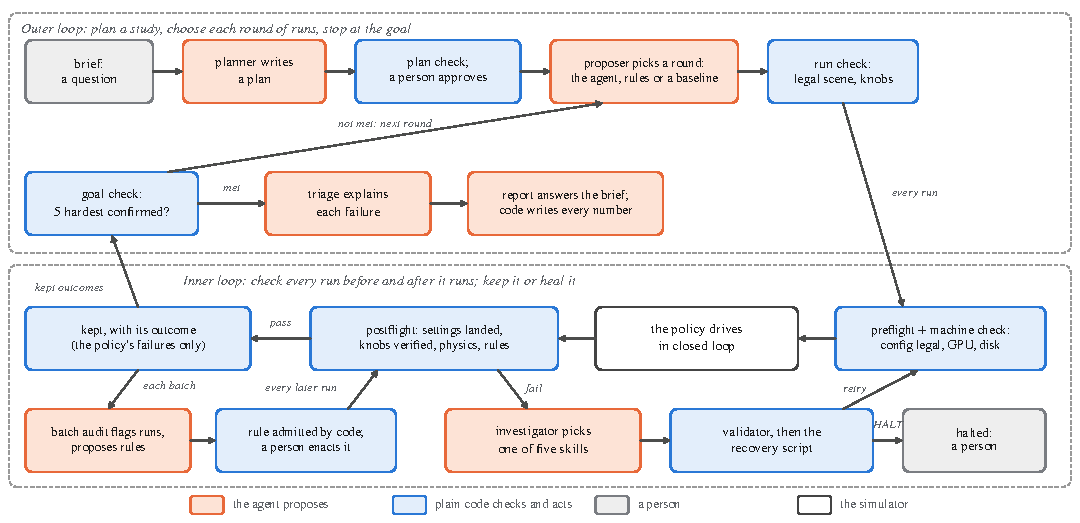
\includegraphics[width=\textwidth]{figures/fig_framework.pdf}
\caption{The framework. Top band, the outer loop: a brief becomes a checked plan, a proposer picks each round of runs, and the goal check decides when to stop; each failure is then triaged and a report answers the brief. Bottom band, the inner loop: each run is checked before and after it runs and kept with its outcome or, if it fails, healed. Orange: the agent proposes; blue: plain code checks and acts; grey: a person.}
\label{fig:system}
\end{figure*}

\subsection{Framework Overview}\label{sec:overview}
\guide{Present Fig.~\ref{fig:system} as a whole: a brief comes in, a checked plan sets up a study, the outer loop picks each round of runs, the inner loop runs, checks and heals every run, kept outcomes go back to the goal check, and once the goal is met each failure is explained and a report answers the brief. Explain the colors: orange boxes are the agent, which only proposes; blue boxes are plain code, which checks every proposal and acts on it; grey is a person (who writes the brief, approves the plan, enacts a new rule and takes over a halted run). Define a campaign and a study (scenes, knobs, goal, budget). Then the design rule shared by every orange box: a contract with five parts (when code calls it, what it sees, what it may answer from a fixed menu or schema, who checks the answer, and who acts: a script, never the agent). Leave the concrete simulator and scenarios to Sec.~\ref{sec:setup}.}

\subsection{Outer Loop: Planning and Choosing the Next Runs}\label{sec:outer}
\guide{The top band of Fig.~\ref{fig:system}, left to right. The planner turns the brief into scenes, knobs, rounds and a goal, and code checks the plan before a person approves it. The proposer (rules, a baseline, or the agent) picks each round; every proposed run is checked before it is queued (a candidate scene, legal knob values) and anything else is dropped. Kept outcomes return to the goal check: define a confirmed hardest case precisely (a setting whose failure rate is surely above one half, by a confidence interval over its repeats, at most one per scene), since Sec.~\ref{sec:results} counts them. List the search methods that can act as the proposer (rules, random search with repeats, Optuna~\cite{akiba2019optuna} with repeats, and the agent alone or combined with either), all under the same gate and budget.}

\subsection{Inner Loop: Running and Checking Each Run}\label{sec:gate}
\guide{The upper row of the bottom band of Fig.~\ref{fig:system}. Each run passes checks before launch, runs in closed loop, and passes checks after it, in a fixed order; it is kept only if the requested scenario provably happened (read back from its logs) and its motion is physically plausible. Stress that code, not the model, decides that a run failed and names the reason. Define the outcome a kept run carries: a failure counts only if the policy is at fault after it takes over. Then the batch audit and how new checks are learned: the auditor flags runs that are wrong in the same way and proposes rules; code admits a rule only if it catches the flagged runs and fires on no clean run; a person enacts it; from then on it is checked on every run \emph{(Fig.~\ref{fig:system} does not show the auditor yet; add it when the figure is redrawn)}.}

\subsection{Inner Loop: Healing Failed Runs}\label{sec:diagnose}
\guide{The lower row of the bottom band of Fig.~\ref{fig:system}, zoomed in twice. Fig.~\ref{fig:contract} zooms into that row: the five steps around the investigator, of which only the third is the agent. Fig.~\ref{fig:io} zooms further into steps 2 and 3: what the agent is given and what it may return. Walk through them: the diagnose contract is called only on a failed run and sees the failure status, the config, the attempt count, error lines and a machine snapshot, with read-only tools. It answers one of five skills; for each, say what the recovery script does with it and when the validator accepts it. RE-RUN queues the same run again. CONFIGURE changes how the run executes (context length, scene file, where the traffic model runs), never what it measures. RESTART\_CLEANUP takes down this run's containers, then reruns it. CLEANUP\_ENV clears leftovers from the whole machine; it is the only fix allowed when the machine was not ready, once per run. HALT stops the run for a person; it is always accepted, and after a machine failure it stops the whole batch. Every skill but HALT needs an attempt left. Code restricts the choice before launch and through the attempt budget, while after launch every skill is allowed and the choice is the agent's (for example, halting every physically wrong run). Note that the tools are read-only by permission, not by instruction. End with the exhaustive check of every answer the agent could give. \emph{Redraw Fig.~\ref{fig:contract} in the paper's style: title it by its role, the inner loop's investigator, and show only the five steps; campaign counts belong in Sec.~\ref{sec:healing}, not in this figure.}}

\begin{figure*}[t]
\centering
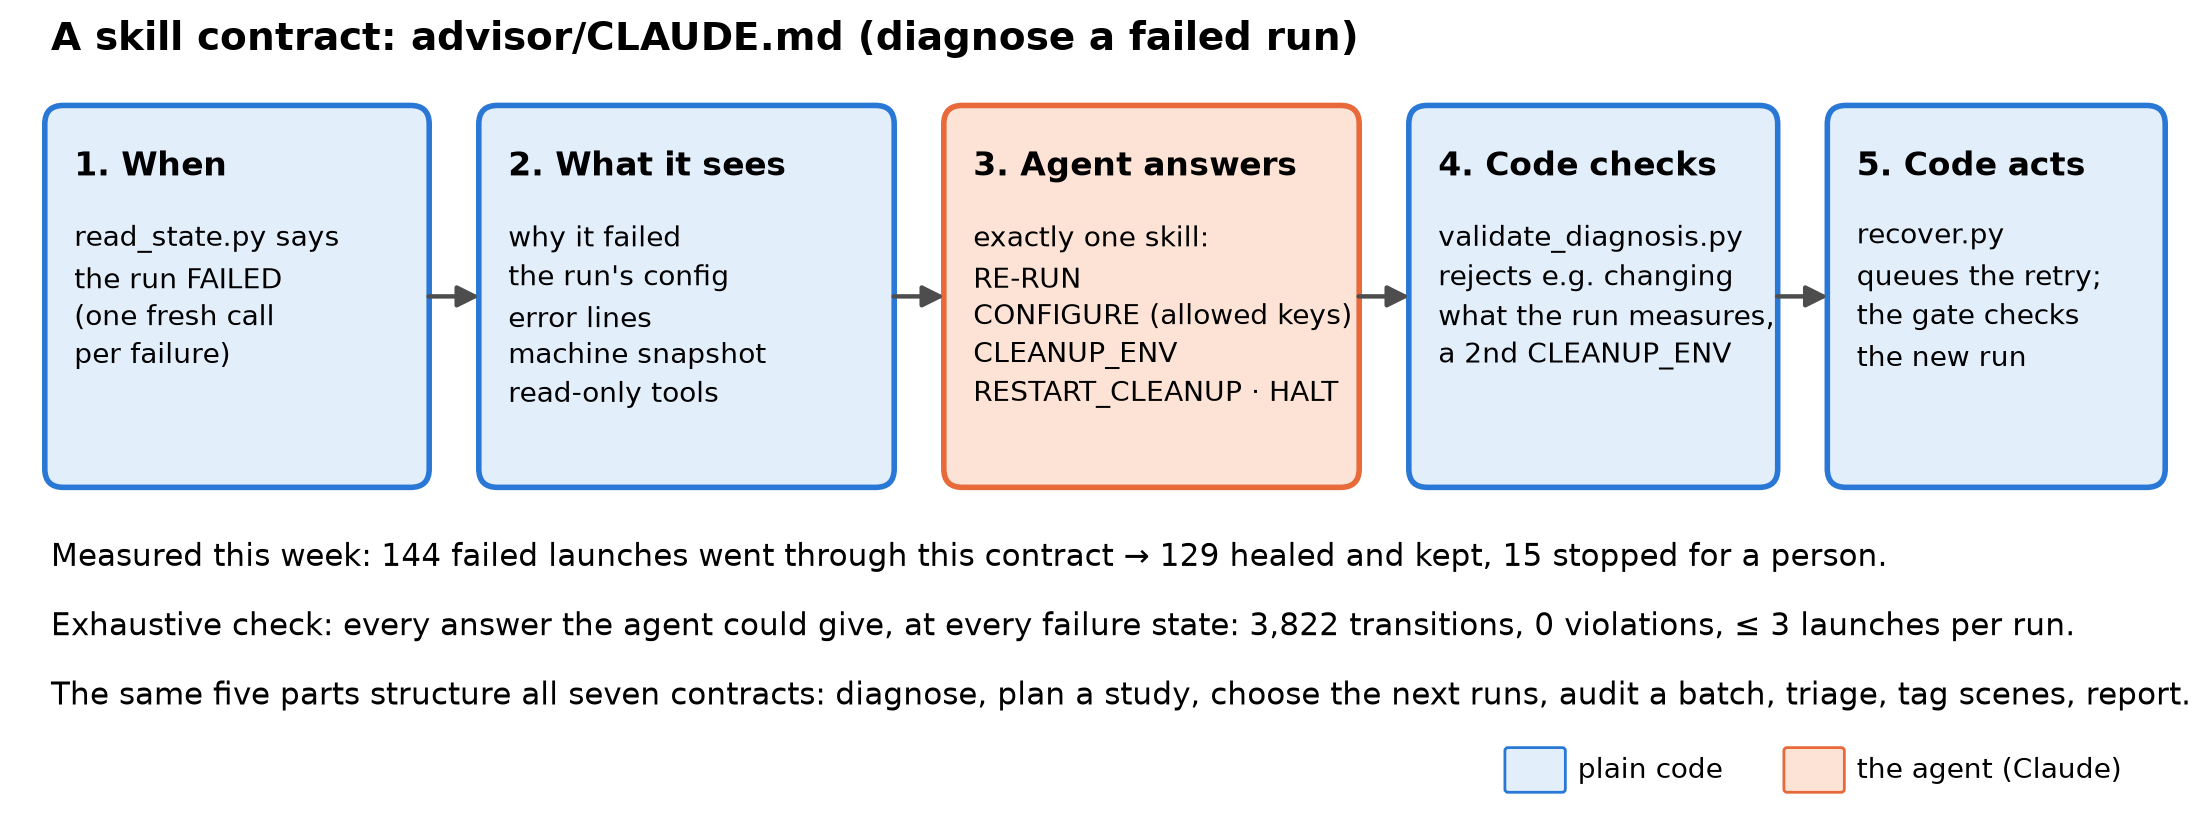
\includegraphics[width=\textwidth]{figures/fig_skill_contract.png}
\caption{A zoom into the lower row of Fig.~\ref{fig:system}: the five steps around the inner loop's investigator, which chooses how to recover a failed run. Only step 3 is the agent; code decides when it is called and what it sees, checks its answer, and acts on it. The planner, the proposer and triage follow the same five steps with their own inputs and menus.}
\label{fig:contract}
\end{figure*}

\guide{\emph{FIGURE TO ADD (Fig.~\ref{fig:io}, a further zoom into steps 2 and 3 of Fig.~\ref{fig:contract}; it does not exist yet): a block diagram of the diagnose agent's input and output. Left, the input that code packs as JSON: the failure status, the config, the attempt count and its limit, up to 15 error lines, and the machine snapshot. Middle, the agent: one fresh call whose system prompt is the contract, with read-only tools (the run's log and folder, the container list, GPU memory, disk). Right, its output: one skill and its params, from a fixed schema with no free text; then the validator (accept or reject) and what the recovery script does for each skill. Along the bottom, one real failure traced through it, e.g.\ a GPU out-of-memory crash where the agent checked GPU memory and containers, answered RE-RUN, was accepted, and the run was kept on its second attempt. Agent orange, code blue, as in Fig.~\ref{fig:system}.}}

\begin{figure*}[t]
\centering
\fbox{\parbox[c][1.3in][c]{0.95\textwidth}{\centering\textit{Placeholder: the investigator's input and output (to be drawn).}}}
\caption{The investigator's input and output (to be drawn): what code packs for it, the agent's one call with read-only tools, and its answer from a fixed schema, followed by the validator and the recovery script; one real failure traced along the bottom.}
\label{fig:io}
\end{figure*}

\subsection{Closing a Study: Triage and Report}\label{sec:explain}
\guide{The right end of the top band of Fig.~\ref{fig:system}. Triage: for each failed run the agent sees frames before the failure and the metrics, and answers a cause from a fixed list and whether the policy was at fault; counts over these answers are computed by code. Report: the agent answers the brief by citing setting ids; code writes every number, and a report with a hand-written count is refused.}

% ---------------------------------------------------------------------------
\section{Simulation Results}\label{sec:results}
\guide{\textbf{Opening paragraph.} Three or four sentences: the setup (\ref{sec:setup}), then one claim per subsection: valid runs (\ref{sec:validity}), unattended self-healing (\ref{sec:healing}), faster corner-case discovery (\ref{sec:discovery}), trustworthy triage (\ref{sec:triage}), findings on the policy (\ref{sec:cases}). No numbers here. \emph{Add a small table mapping each subsection to the part of Fig.~\ref{fig:system} it tests: \ref{sec:validity}, the checks before and after each run, plus the batch audit; \ref{sec:healing}, the investigator, validator and recovery; \ref{sec:discovery}, the proposer and the goal check (only the proposer changes between methods); \ref{sec:triage}, triage; \ref{sec:cases}, the report, i.e.\ what the whole pipeline produced.}}

\subsection{Simulation Setup}\label{sec:setup}
\guide{Two parts. \textbf{Simulation:} the simulator and policy (AlpaSim~\cite{alpasim}, VaVAM~\cite{bartoccioni2025vavam}, linear MPC tracking, replayed traffic; planning at 2 Hz and 10 Hz), the knobs, the test scenarios (studies mapped to Euro NCAP tests~\cite{euroncap2023vru,euroncap2023c2c}), repeats and run budgets per method, the metrics (confirmed hardest cases, runs to reach the goal, model time) and the statistical tests. \textbf{Computing environment:} one workstation (GPU model and memory, CPU, RAM, disk, operating system) running two simulations at once on its single GPU; the simulator in containers, with the added retiming and seeding hooks off by default; the agent's model and how it is called (one fresh headless call per decision, read-only tools, time per call); run time (simulated seconds and wall-clock per run at each planning rate, total GPU hours). \emph{Confirm the exact hardware and software versions for the whole campaign; a short table is a common way to report them.}}

\subsection{Validity of Kept Runs}\label{sec:validity}
\guide{Test whether every kept run is real data, in both directions: bad runs must be caught and good runs kept. (1) Planted faults: in three campaigns, runs were broken on purpose in ways that still end normally (deleted or corrupted results, a requested setting silently dropped, the recorded human driving the whole run, no controller in the loop). Count the invalid runs kept with no gate, with the per-run gate, and with the batch audit added, and give an upper bound on the share that could still slip through. Say which faults only the batch audit catches and why (they look the same in every run of a batch). (2) False alarms: the physics check on clean runs (none should be thrown away) and on runs with silent motion faults (all should be caught). (3) Close by noting that every later result uses kept runs only. \emph{Add a small table, generated from the data: invalid runs kept per planted-fault campaign with no gate, the per-run gate, and gate + audit. No figure is needed.}}

\subsection{Self-Healing in Unattended Operation}\label{sec:healing}
\guide{Test whether the agent keeps a long campaign running without a person, using every failed launch of the whole campaign. (1) Scale and outcome: runs asked for, runs kept on the first try, launches that failed and went to the agent, and how many of those were healed or stopped for a person (Fig.~\ref{fig:healing}). (2) What the agent chose: for each kind of failure, the skill it picked and how the run ended; every answer passed the validator, and every retry ran exactly the settings asked for. (3) Honest accounting: most heals are out-of-memory crashes answered by a plain rerun, which a retry script would also do; the agent's value is in the rest, such as halting runs that failed the physics check instead of rerunning them and clearing a machine that was not ready. (4) Against a retry script: on the planted-fault campaigns, the same faults handled by a fixed script, by the agent without tools, and by the agent with read-only tools; compare valid runs kept, launches used and runs stopped, and note where the agent without tools fails (results missing despite a normal exit). Report the agent's time per decision. \emph{Regenerate Fig.~\ref{fig:healing} from the final data before submission. Give (4) as a few numbers in the text, or a small table if space allows.}}

\begin{figure*}[t]
\centering
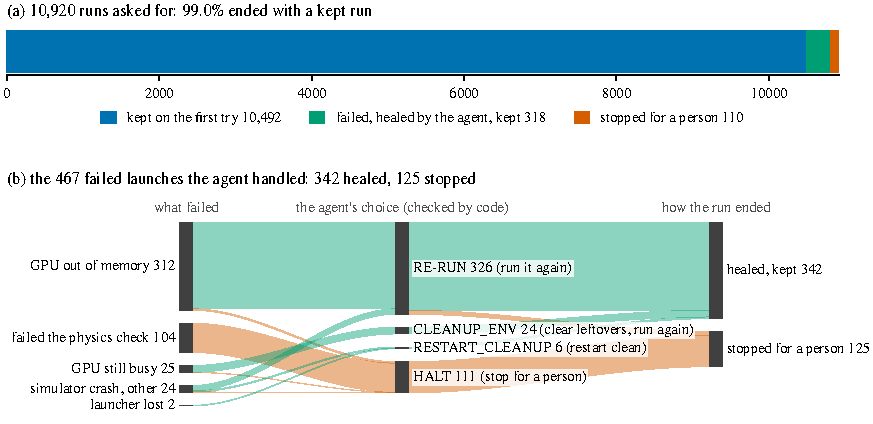
\includegraphics[width=0.8\textwidth]{figures/fig_healing_flow.pdf}
\caption{Every run asked for, and every failed launch the agent handled: what failed, the skill it chose, how the run ended. Each failure is listed with its raw evidence in the released failure ledger.}
\label{fig:healing}
\end{figure*}

\subsection{Corner-Case Discovery Across Search Methods}\label{sec:discovery}
\guide{Test whether letting the agent choose the next tests finds and confirms the hardest cases sooner, at an equal budget under the same gate. (1) The comparison: each method replaces only the proposer; studies, budgets, rounds and goal stay the same; each method runs several repeats. Report confirmed hardest cases at the budget and runs to reach the goal (Fig.~\ref{fig:discovery}, Table~\ref{tab:methods}). (2) Main result first: the three-knob study, where failures are rare, with five repeats and comparisons planned before the extra repeats were run; then lane keeping, a study the second AI version was not built on; then the car scenes and the pedestrian study, where failures are common. (3) The pattern: the agent's lead grows as failures get rarer, and where failures are common it has no edge (say so); Optuna alone does no better than random search with repeats; the agent restricted to the rules' candidates does well only where those candidates are good. Explain it by where each method looked: the rules start in the middle of each knob's range and step locally, random search and Optuna spread runs thin, the agent uses the physics stated in the brief and repeats what fails. (4) Counting decides the ranking: under a naive collision count (contacts begun before the hand-off, rear-ends by replayed traffic) the ranking changes; show it briefly. \emph{Fig.~\ref{fig:discovery} and Table~\ref{tab:methods} are placeholders with the three 10 Hz studies only; add the three-knob study and lane keeping, ordered from rare to common failures. Compute every test statistic with code.}}

\begin{figure*}[t]
\centering
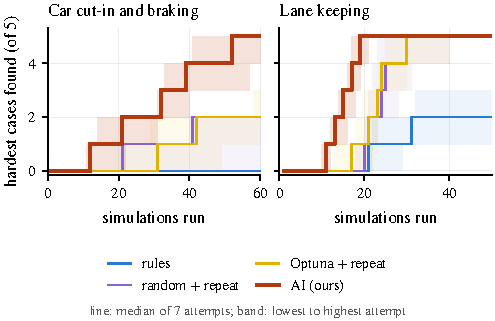
\includegraphics[width=\textwidth]{figures/fig_discovery.pdf}
\caption{Confirmed hardest cases against kept runs, per method: median and range over repeats.}
\label{fig:discovery}
\end{figure*}
\begin{table}[t]
\caption{Search methods at an equal budget per study.}
\label{tab:methods}
\centering\footnotesize
\setlength{\tabcolsep}{2.5pt}
\begin{tabular}{@{}lccccc@{}}
\toprule
 & \multicolumn{2}{c}{Unseen studies, 2\,Hz} & \multicolumn{2}{c}{Method studies, 10\,Hz} & \\
\cmidrule(lr){2-3}\cmidrule(lr){4-5}
 & Cut-in, braking & Lane keeping & Car scenes & Pedestrian & Model \\
Method & confirmed & runs to goal & confirmed & runs to goal & s/arm \\
\midrule
rules & 0/25 & never & 6/30 & 25 (25) & -- \\
random + repeat & 7/25 & 30 (23--31) & 10/30 & 32 (31--32) & -- \\
Optuna + repeat & 10/25 & 32 (25--40) & 13/30 & 31 (25--33) & -- \\
hybrid (rules + AI) & 5/15 & 1 of 3 reached, 45 & 17/30 & 24 (24--28) & 89 \\
Optuna + AI & 13/25 & 20 (18--21) & 13/30 & 21 (20--21) & 97 \\
AI, first prompt & 17/25 & 20 (19--22) & 13/30 & 37 (28--40) & 101 \\
AI (ours) & 24/25 & 18 (17--21) & -- & -- & 88 \\
hybrid, revised prompt & 7/15 & 2 of 3 reached, 39--43 & -- & -- & 118 \\
\bottomrule
\end{tabular}
\\[2pt]\parbox{\columnwidth}{\scriptsize Confirmed: hardest settings confirmed by repeats, summed over repeats (5 per repeat). Runs to goal: kept runs until all 5 were confirmed, median (range); `never' if no repeat got there. Cut-in, braking: a car cutting in or braking ahead, three knobs, rare failures. Car scenes: car cutting in and car ahead braking. Repeats per arm: unseen studies 3--5, 10\,Hz studies 3. Contacts with a car the retiming held still are not counted. Model: median seconds of model calls per arm.}
\end{table}


\subsection{Reliability of Failure Triage}\label{sec:triage}
\guide{Check how far the agent's explanation of each failure can be trusted, against code and against people. (1) Against a rule in code that decides who closed the gap at the contact: on the collision failures of the car studies, how often the rule and triage agree on whether the ego or the other car was to blame, and where they disagree, including nearly identical contacts that triage labelled differently. (2) Against people: a person labels who caused each of 60 randomly drawn crashes without seeing the scorer or the triage; report agreement and Cohen's kappa with the scorer and with the triage. (3) A person marks each case card as making sense or not, including the hardest cases where triage and the scorer disagree. Close with what the failure types in Sec.~\ref{sec:cases} can and cannot be trusted for. \emph{Part (1) is done; (2) and (3) wait for the human labels and verdicts. Report (1)--(3) in one small table (check, cases, agreement, kappa); no figure is needed.}}

\subsection{Failures Found in the VaVAM Policy}\label{sec:cases}
\guide{A case study of what the campaign revealed about the policy under test, in four parts. (1) Hardest cases: for each case in Fig.~\ref{fig:cases}, the setting that triggered it, what the ego did from the hand-off to the failure, and why it is the policy's fault. (2) Failure types: most failures are steering into another road user or leaving the road, few are failures to brake, although the studies were built around braking; the types come from the triage checked in Sec.~\ref{sec:triage}. (3) The left drift: after the hand-off the ego moves steadily left of the human's path in nearly every run, never right; with the camera image and the plan mirrored it drifts right, so the bias is the model's, not the simulator's. Most hardest cases are this drift meeting traffic or the road edge. (4) The pedestrian stressor: retiming the pedestrian alone rarely causes failures; a faster ego at the hand-off does. Note that some pedestrian failures happen far from the recorded path, where rendering is less reliable, and that these are flagged. \emph{Fig.~\ref{fig:cases} covers only part (1). Add a column-width figure for (3): the ego's lateral offset from the human's path against time since the hand-off, over all kept runs, with the mirrored runs drifting the other way. Give (2) as shares in the text; if space allows, a small table of failure types by study instead of a chart. No other table is needed here. Move the note printed inside Fig.~\ref{fig:cases} into its caption, and prefer cases that show the drift.}}

\begin{figure*}[t]
\centering
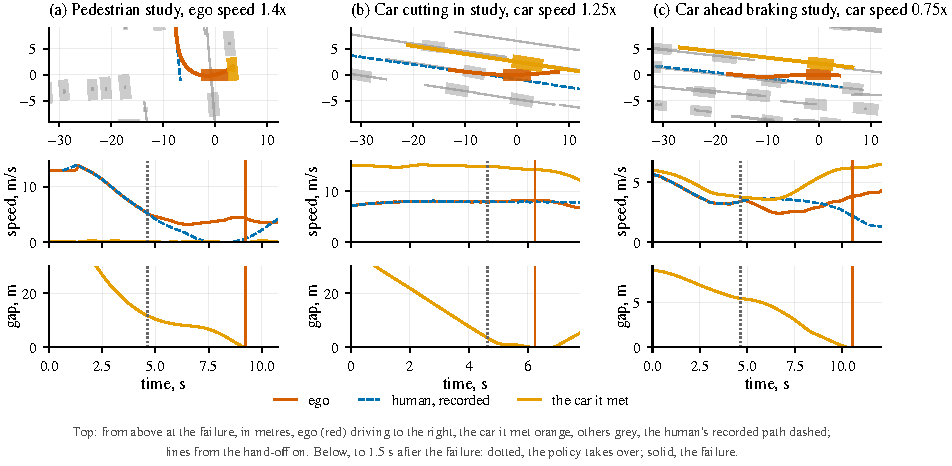
\includegraphics[width=0.9\textwidth]{figures/fig_cases.pdf}
\caption{Three confirmed hardest cases, from above and as speed and gap over time.}
\label{fig:cases}
\end{figure*}

% ---------------------------------------------------------------------------
\section{Conclusion}\label{sec:conclusion}
\guide{\textbf{Paragraph 1: summary.} Restate the two main claims in a few sentences: an agent can run stress testing of a driving policy end to end, unattended, when each action is a checked choice from a fixed menu; and letting it choose the next tests pays off most where failures are rare. Say where the code and data are released.}

\guide{\textbf{Paragraph 2: limitations and future work.} Pair each limitation with the direction that addresses it: one policy under test (test more end-to-end policies); replayed traffic does not react (use reactive traffic); few scenes for some maneuvers (add more scenario types); few repeats per method (run more repeats, and try other models as the agent). Also state the limitations with no direction yet: rendering is less certain far from the recording, and the human check of the scoring is still pending. End with the confirmed hardest cases reused as regression tests.}

\section*{AI Use Disclosure}
\guide{Required by IEEE: state that the agent under study is Claude, and disclose any AI assistance in the code and the writing.}

\guide{\emph{Cut the references to about 15. Keep the closest work (EvoDrive, PlannerForge, LLM-attacker, EC-Detector, ARISE), the testing roots (NADE, D2RL, AST), the tools used (AlpaSim, VaVAM, Optuna), and one or two each on unreliable agent results and safe agents.}}
\bibliographystyle{IEEEtran}
\bibliography{refs}

\end{document}
